\documentclass[12pt,reqno,final]{amsart}\usepackage[]{graphicx}\usepackage[]{color}
%% maxwidth is the original width if it is less than linewidth
%% otherwise use linewidth (to make sure the graphics do not exceed the margin)
\makeatletter
\def\maxwidth{ %
  \ifdim\Gin@nat@width>\linewidth
    \linewidth
  \else
    \Gin@nat@width
  \fi
}
\makeatother

\definecolor{fgcolor}{rgb}{0.345, 0.345, 0.345}
\newcommand{\hlnum}[1]{\textcolor[rgb]{0.686,0.059,0.569}{#1}}%
\newcommand{\hlstr}[1]{\textcolor[rgb]{0.192,0.494,0.8}{#1}}%
\newcommand{\hlcom}[1]{\textcolor[rgb]{0.678,0.584,0.686}{\textit{#1}}}%
\newcommand{\hlopt}[1]{\textcolor[rgb]{0,0,0}{#1}}%
\newcommand{\hlstd}[1]{\textcolor[rgb]{0.345,0.345,0.345}{#1}}%
\newcommand{\hlkwa}[1]{\textcolor[rgb]{0.161,0.373,0.58}{\textbf{#1}}}%
\newcommand{\hlkwb}[1]{\textcolor[rgb]{0.69,0.353,0.396}{#1}}%
\newcommand{\hlkwc}[1]{\textcolor[rgb]{0.333,0.667,0.333}{#1}}%
\newcommand{\hlkwd}[1]{\textcolor[rgb]{0.737,0.353,0.396}{\textbf{#1}}}%
\let\hlipl\hlkwb

\usepackage{framed}
\makeatletter
\newenvironment{kframe}{%
 \def\at@end@of@kframe{}%
 \ifinner\ifhmode%
  \def\at@end@of@kframe{\end{minipage}}%
  \begin{minipage}{\columnwidth}%
 \fi\fi%
 \def\FrameCommand##1{\hskip\@totalleftmargin \hskip-\fboxsep
 \colorbox{shadecolor}{##1}\hskip-\fboxsep
     % There is no \\@totalrightmargin, so:
     \hskip-\linewidth \hskip-\@totalleftmargin \hskip\columnwidth}%
 \MakeFramed {\advance\hsize-\width
   \@totalleftmargin\z@ \linewidth\hsize
   \@setminipage}}%
 {\par\unskip\endMakeFramed%
 \at@end@of@kframe}
\makeatother

\definecolor{shadecolor}{rgb}{.97, .97, .97}
\definecolor{messagecolor}{rgb}{0, 0, 0}
\definecolor{warningcolor}{rgb}{1, 0, 1}
\definecolor{errorcolor}{rgb}{1, 0, 0}
\newenvironment{knitrout}{}{} % an empty environment to be redefined in TeX

\usepackage{alltt}
\usepackage[round,numbers,sort&compress]{natbib}
\usepackage{graphicx}
\usepackage{times}
\usepackage{rotating}
\usepackage{subfig}

\title[]{}

\setlength{\textwidth}{6.25in}
\setlength{\textheight}{8.75in}
\setlength{\evensidemargin}{0in}
\setlength{\oddsidemargin}{0in}
\setlength{\topmargin}{-.35in}
\setlength{\parskip}{.1in}
\setlength{\parindent}{0.0in}

\theoremstyle{plain}
\newtheorem{thm}{Theorem}
\newtheorem{corol}[thm]{Corollary}
\newtheorem{prop}[thm]{Proposition}
\newtheorem{lemma}[thm]{Lemma}
\newtheorem{defn}[thm]{Definition}
\newtheorem{hyp}[thm]{Hypothesis}
\newtheorem{example}[thm]{Example}
\newtheorem{conj}[thm]{Conjecture}
\newtheorem{algorithm}[thm]{Algorithm}
\newtheorem{remark}{Remark}
\renewcommand\thethm{\arabic{thm}}
\renewcommand{\theremark}{}

\numberwithin{equation}{part}
\renewcommand\theequation{\arabic{equation}}
\renewcommand\thesection{\arabic{section}}
\renewcommand\thesubsection{\thesection.\arabic{subsection}}
\renewcommand\thefigure{\arabic{figure}}
\renewcommand\thetable{\arabic{table}}
\renewcommand\thefootnote{\arabic{footnote}}
\IfFileExists{upquote.sty}{\usepackage{upquote}}{}
\begin{document}

\maketitle

This documents my exploration of the differences between \texttt{OUwie} and \texttt{ouch} when each is asked to fit OU models with a single $\alpha$ and $\sigma$ operating on the entire tree.
The motivation for this is that I noticed that the parameter estimates and likelihoods reached by \texttt{OUwie} and \texttt{ouch} are often quite different.
I originally did this is 2014, but wanted to update it now to explore how the programs differ from one another now.

The procedure I will follow here is very straightforward: generate Yule trees of different sizes; specify two selective regimes arising out of the branching event at the root, so that there is a single monophyletic clade in each selective regime - this is the simplest possible multiple-optimum OU scenario; simulate phenotypic data with a known $\alpha$ and $\sigma$; fit an OU model to the phenotypic data and tree using both \texttt{OUwie} and \texttt{ouch} and record the
parameter estimates and likelihoods.

Trees were generated by assuming that branching follows a Poisson process, so that branching events are exponentially distributed. To generate trees of different sizes, I set the rate parameter of the exponential distribution to a value of 0.3 and found random number generator seeds that would generate trees of size from 10 to 100 tips, with the only constraint being that the smaller of the two clades originating at the root had at least 1/3 of the total tip species.
This guarantees that both selective regimes are reasonably well-represented, thereby improving both power and parameter estimates.

Phenotypic data was generated assuming $\alpha=3$ and $\sigma^2=1$, with selective optima of $\theta_1=-1$ and $\theta_2=1$. The root was always assumed to be in regime 1. For any given tree size, 20 different phenotypic datasets were generated and fit to the OU model.
This allows me to calculate how bias/variance in parameter estimates differ between the two algorithms.
All of the code, including random number generator seeds, needed to reproduce the results shown here can be found at the end of this document.

\begin{knitrout}
\definecolor{shadecolor}{rgb}{0.969, 0.969, 0.969}\color{fgcolor}\begin{kframe}


{\ttfamily\noindent\itshape\color{messagecolor}{\#\# `geom\_smooth()` using method = 'gam' and formula 'y \textasciitilde{} s(x, bs = "{}cs"{})'}}\end{kframe}\begin{figure}
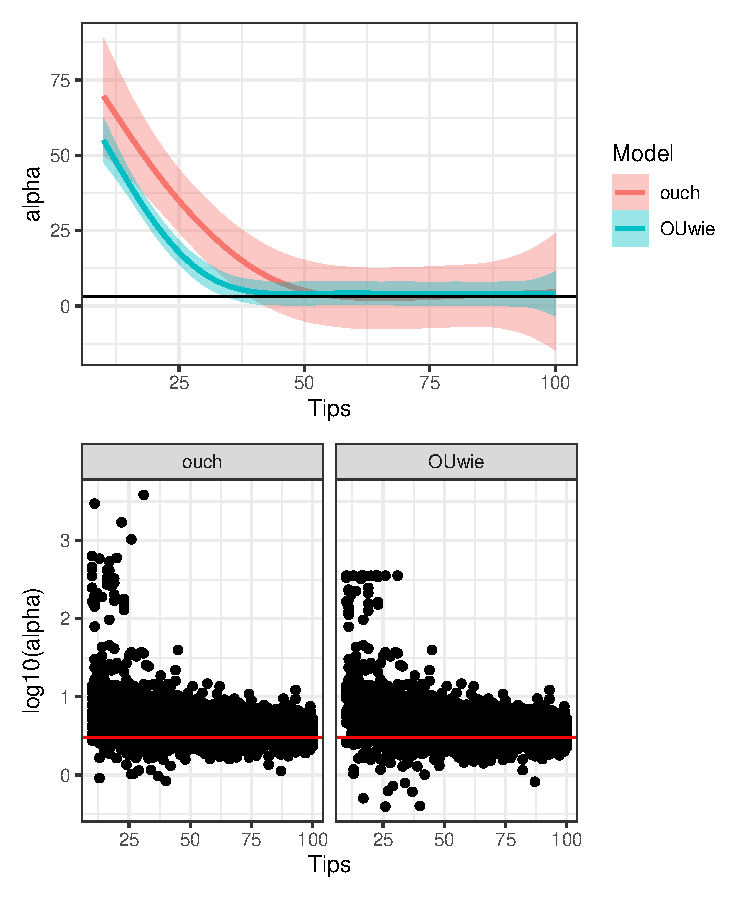
\includegraphics[width=\maxwidth]{figure/unnamed-chunk-1-1} \caption{Comparing the $\alpha$ estimates of \texttt{ouch} and \texttt{OUwie} for trees of 10-100 tips. In the top panel, the lines and shaded region come from fitting a generalized additive model to the $\alpha$ estimates, with the size of the tree as the dependent variable. The line shows the expectation of the GAM, whereas the shaded regions capture the variability across the 20 stochastically generated phenotypic datasets. The black line shows the true $\alpha$ value. From this figure, it appears that the estimates are converging on the true value, but the error around the \texttt{ouch} estimates is higher than for \texttt{OUwie}. However, an examination of the estimates for each dataset (bottom panels) shows that variability is actually still fairly large. It is clear, however, that neither method is particularly good or bad at estimating $\alpha$. If anything, \texttt{OUwie} is slightly better than \texttt{ouch}, which is a change from 2014, when I did this analysis.}\label{fig:unnamed-chunk-1}
\end{figure}


\end{knitrout}

\begin{knitrout}
\definecolor{shadecolor}{rgb}{0.969, 0.969, 0.969}\color{fgcolor}\begin{kframe}


{\ttfamily\noindent\itshape\color{messagecolor}{\#\# `geom\_smooth()` using method = 'gam' and formula 'y \textasciitilde{} s(x, bs = "{}cs"{})'}}\end{kframe}\begin{figure}
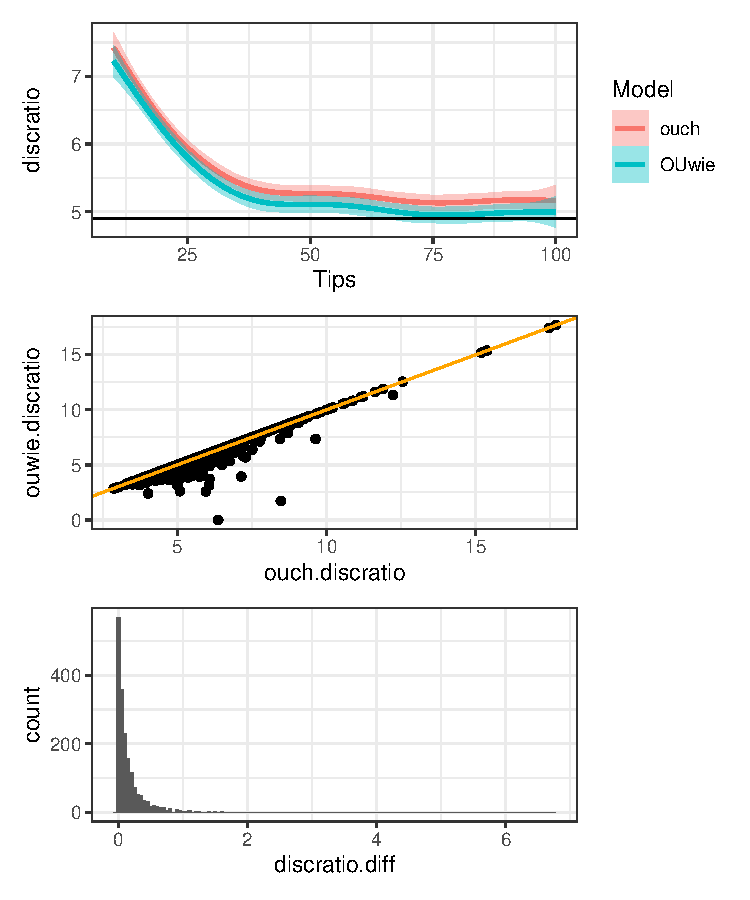
\includegraphics[width=\maxwidth]{figure/unnamed-chunk-2-1} \caption{Estimates of the discriminability ratio, $\sqrt{2\alpha}\Delta\theta/\sigma$ (Cressler, Butler, and King 2015). This dimensionless combination of parameters may be better estimated than any individual parameter. This dimensionless parameter also captures the linked ability to estimate the selective optima, selection strength, and drift. You can see from all three panels that \texttt{ouch} and \texttt{OUwie} often estimate this parameter nearly identically: the top panel shows results from a generalized additive model fit to the estimates for each number of tips; the middle panel shows a scatterplot of the estimates for each method; the bottom panel shows a histogram of the difference between the \texttt{ouch} estimate and the \texttt{OUwie} estimate. Interestingly, the estimate returned by \texttt{ouch} is always larger than the estimate returned by \texttt{OUwie}.}\label{fig:unnamed-chunk-2}
\end{figure}


\end{knitrout}

\begin{knitrout}
\definecolor{shadecolor}{rgb}{0.969, 0.969, 0.969}\color{fgcolor}\begin{figure}
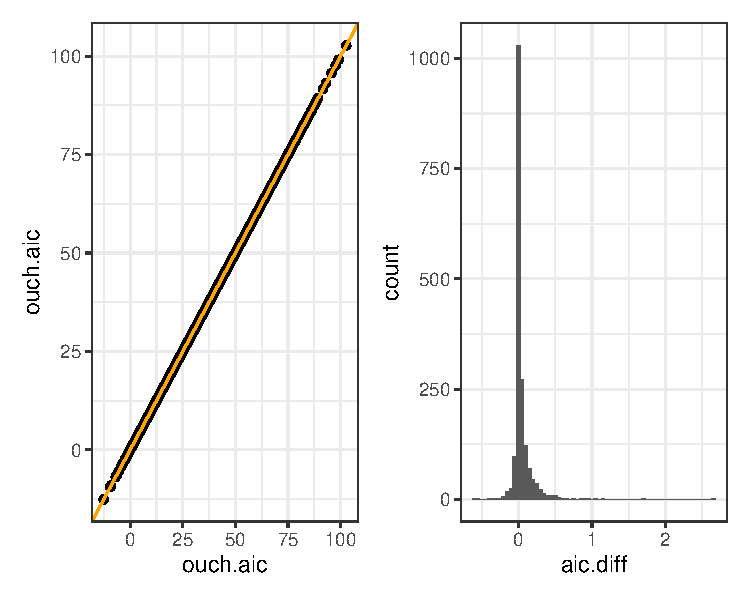
\includegraphics[width=\maxwidth]{figure/unnamed-chunk-3-1} \caption{Estimated AICs for \texttt{ouch} and \texttt{OUwie} are essentially identical. The histogram shows the difference between the AIC of the parameters estimated by \texttt{ouch} and the AIC of the \texttt{OUwie} parameter estimates; positive values suggest that 	exttt{OUwie} has found parameter estimates with a higher likelihood.}\label{fig:unnamed-chunk-3}
\end{figure}


\end{knitrout}

\newpage

\begin{knitrout}
\definecolor{shadecolor}{rgb}{0.969, 0.969, 0.969}\color{fgcolor}\begin{kframe}
\begin{alltt}
\hlkwd{require}\hlstd{(ouch)}
\hlcom{## Creates an ouchtree object.}
\hlcom{##}
\hlcom{## 'waittime' must be specified by the user, and is the}
\hlcom{## expected time to a branching event, assuming the branching}
\hlcom{## follows a Poisson process (that is, that branching events}
\hlcom{## are exponentially distributed)}
\hlcom{##}
\hlcom{## 'endtime' must also be specified and determines how long to}
\hlcom{## let the branching process proceed.}
\hlcom{##}
\hlcom{## The smaller the value of waittime, or the larger the value}
\hlcom{## of endtime, the larger the tree that will be produced. If}
\hlcom{## only these two variables are set, the tree that is produced}
\hlcom{## will be ultrametric; specifically, it will be a Yule tree,}
\hlcom{## corresponding to a pure birth process.}
\hlcom{##}
\hlcom{## 'time' can also be specified, setting the time of the root}
\hlcom{## node.}

\hlcom{## A birth-death branching process can be simulated by setting}
\hlcom{## the value of extrate, which determines the rate at which}
\hlcom{## lineages go extinct. This rate is also assumed to be}
\hlcom{## exponentially distributed.}
\hlcom{##}
\hlstd{gen.tree} \hlkwb{<-} \hlkwa{function}\hlstd{(}\hlkwc{waittime}\hlstd{,} \hlkwc{endtime}\hlstd{,}
                     \hlkwc{time} \hlstd{=} \hlnum{0}\hlstd{,} \hlkwc{extrate} \hlstd{=} \hlnum{0}\hlstd{,}
                     \hlkwc{anc.node} \hlstd{=} \hlnum{NA}\hlstd{,} \hlkwc{tree}\hlstd{) \{}
    \hlkwa{if} \hlstd{(}\hlkwd{missing}\hlstd{(tree))}
        \hlstd{tree} \hlkwb{<-} \hlkwd{matrix}\hlstd{(}\hlnum{NA}\hlstd{,}\hlnum{0}\hlstd{,}\hlnum{3}\hlstd{,}
                       \hlkwc{dimnames}\hlstd{=}\hlkwd{list}\hlstd{(}\hlkwa{NULL}\hlstd{,}\hlkwd{c}\hlstd{(}\hlstr{"node"}\hlstd{,}\hlstr{"ancestor"}\hlstd{,}\hlstr{"time"}\hlstd{)))}
    \hlstd{curr.node} \hlkwb{<-} \hlkwd{nrow}\hlstd{(tree)}\hlopt{+}\hlnum{1}
    \hlkwa{if} \hlstd{(time} \hlopt{<} \hlstd{endtime) \{}
        \hlstd{tree} \hlkwb{<-} \hlkwd{rbind}\hlstd{(tree,}\hlkwd{c}\hlstd{(curr.node,anc.node,time))}
        \hlstd{extinct.time} \hlkwb{<-} \hlkwa{if} \hlstd{(extrate} \hlopt{>} \hlnum{0}\hlstd{) \{}
            \hlstd{time}\hlopt{+}\hlkwd{rexp}\hlstd{(}\hlnum{2}\hlstd{,}\hlkwc{rate}\hlstd{=extrate)}
        \hlstd{\}} \hlkwa{else} \hlstd{\{}
            \hlkwd{c}\hlstd{(}\hlnum{Inf}\hlstd{,}\hlnum{Inf}\hlstd{)}
        \hlstd{\}}
        \hlstd{time} \hlkwb{<-} \hlkwd{pmin}\hlstd{(time}\hlopt{+}\hlkwd{rexp}\hlstd{(}\hlnum{2}\hlstd{,}\hlkwc{rate}\hlstd{=}\hlnum{1}\hlopt{/}\hlstd{waittime),endtime)}
        \hlkwa{for} \hlstd{(k} \hlkwa{in} \hlnum{1}\hlopt{:}\hlnum{2}\hlstd{) \{}
            \hlkwa{if} \hlstd{(time[k]} \hlopt{<} \hlstd{extinct.time[k]) \{}
                \hlstd{tree} \hlkwb{<-} \hlkwd{Recall}\hlstd{(}\hlkwc{time}\hlstd{=time[k],}
                               \hlkwc{waittime}\hlstd{=waittime,}\hlkwc{endtime}\hlstd{=endtime,}\hlkwc{extrate}\hlstd{=extrate,}\hlkwc{anc.node}\hlstd{=curr.node,}\hlkwc{tree}\hlstd{=tree)}
            \hlstd{\}} \hlkwa{else} \hlstd{\{}
                \hlstd{tree} \hlkwb{<-} \hlkwd{rbind}\hlstd{(tree,}\hlkwd{c}\hlstd{(}\hlkwd{nrow}\hlstd{(tree)}\hlopt{+}\hlnum{1}\hlstd{,curr.node,extinct.time[k]))}
            \hlstd{\}}
        \hlstd{\}}
    \hlstd{\}} \hlkwa{else} \hlstd{\{}
        \hlstd{tree} \hlkwb{<-} \hlkwd{rbind}\hlstd{(tree,}\hlkwd{c}\hlstd{(curr.node,anc.node,time))}
    \hlstd{\}}
    \hlkwd{return}\hlstd{(}\hlkwd{as.data.frame}\hlstd{(tree))}
\hlstd{\}}

\hlcom{## Generate phenotypic data according to an Ornstein-Uhlenbeck}
\hlcom{## process, given an ouchtree object specified by tree, regimes}
\hlcom{## specified by regimes, and OU parameters theta, alpha, and sigma.}
\hlcom{## This is done by recursion, which gen.phenotypic.values acting as}
\hlcom{## the "parent" function that calls set.phenotypic.values, the}
\hlcom{## function that is recursed over.}
\hlstd{gen.phenotypic.values} \hlkwb{<-} \hlkwa{function}\hlstd{(}\hlkwc{tree}\hlstd{,} \hlkwc{regimes}\hlstd{,} \hlkwc{theta}\hlstd{,} \hlkwc{alpha}\hlstd{,} \hlkwc{sigma}\hlstd{,} \hlkwc{remove.anc}\hlstd{=}\hlnum{TRUE}\hlstd{) \{}
  \hlkwa{if} \hlstd{(}\hlkwd{class}\hlstd{(tree)} \hlopt{==} \hlstr{'data.frame'}\hlstd{)}
    \hlstd{tree} \hlkwb{<-} \hlkwd{with}\hlstd{(tree,} \hlkwd{ouchtree}\hlstd{(node,ancestor,time))}
  \hlkwa{if} \hlstd{(tree}\hlopt{@}\hlkwc{nnodes} \hlopt{!=} \hlkwd{length}\hlstd{(regimes))}
    \hlkwd{stop}\hlstd{(}\hlstr{'Length of regime specification != number of nodes in tree; each node in tree must be assigned to a regime'}\hlstd{)}
  \hlkwa{if} \hlstd{(}\hlkwd{length}\hlstd{(theta)} \hlopt{!=} \hlkwd{length}\hlstd{(}\hlkwd{levels}\hlstd{(regimes)))}
    \hlkwd{stop}\hlstd{(}\hlstr{'Each regime must have a unique theta value specified as the selective optima'}\hlstd{)}

  \hlstd{root.reg} \hlkwb{<-} \hlkwd{as.numeric}\hlstd{(regimes[}\hlnum{1}\hlstd{])}
  \hlstd{root.pheno} \hlkwb{<-} \hlkwd{calc.root.pheno}\hlstd{(theta[root.reg], alpha, sigma)}
  \hlstd{pheno} \hlkwb{<<-} \hlkwd{vector}\hlstd{(}\hlkwc{mode}\hlstd{=}\hlstr{'numeric'}\hlstd{,} \hlkwc{length}\hlstd{=tree}\hlopt{@}\hlkwc{nnodes}\hlstd{)}
  \hlkwd{set.phenotypic.values}\hlstd{(}\hlkwc{curr.node}\hlstd{=}\hlnum{1}\hlstd{,} \hlkwc{anc.node}\hlstd{=}\hlnum{0}\hlstd{,} \hlkwc{anc.pheno}\hlstd{=root.pheno,} \hlkwc{tree}\hlstd{=tree,} \hlkwc{regimes}\hlstd{=regimes,} \hlkwc{theta}\hlstd{=theta,} \hlkwc{alpha}\hlstd{=alpha,} \hlkwc{sigma}\hlstd{=sigma)}

  \hlcom{## if T, set the phenotypic values of internal nodes to NA}
  \hlkwa{if} \hlstd{(remove.anc}\hlopt{==}\hlstd{T)}
    \hlstd{pheno[}\hlkwd{as.numeric}\hlstd{(}\hlkwd{setdiff}\hlstd{(tree}\hlopt{@}\hlkwc{nodes}\hlstd{, tree}\hlopt{@}\hlkwc{term}\hlstd{))]} \hlkwb{<<-} \hlnum{NA}

  \hlstd{pheno}
\hlstd{\}}
\hlcom{## Calculate the phenotypic value of the ancestral node as being drawn}
\hlcom{## from the stationary distribution of the OU process.}
\hlstd{calc.root.pheno} \hlkwb{<-} \hlkwa{function}\hlstd{(}\hlkwc{theta}\hlstd{,} \hlkwc{alpha}\hlstd{,} \hlkwc{sigma}\hlstd{) \{}
  \hlcom{## mean and variance of stationary distribution}
  \hlstd{mean} \hlkwb{<-} \hlstd{theta}
  \hlstd{var} \hlkwb{<-} \hlstd{sigma}\hlopt{^}\hlnum{2}\hlopt{/}\hlstd{(}\hlnum{2}\hlopt{*}\hlstd{alpha)}
  \hlkwd{rnorm}\hlstd{(}\hlnum{1}\hlstd{,} \hlkwc{mean}\hlstd{=mean,} \hlkwc{sd}\hlstd{=}\hlkwd{sqrt}\hlstd{(var))}
\hlstd{\}}
\hlcom{## This function recursively sets the phenotypic values of the nodes}
\hlcom{## in an ouchtree object specified by tree.  The values are, by}
\hlcom{## default, set for a vector called 'pheno'}
\hlstd{set.phenotypic.values} \hlkwb{<-} \hlkwa{function}\hlstd{(}\hlkwc{curr.node}\hlstd{,} \hlkwc{anc.node}\hlstd{,} \hlkwc{anc.pheno}\hlstd{,} \hlkwc{tree}\hlstd{,} \hlkwc{regimes}\hlstd{,} \hlkwc{theta}\hlstd{,} \hlkwc{alpha}\hlstd{,} \hlkwc{sigma}\hlstd{) \{}
  \hlcom{## set the phenotype of the current node}
  \hlkwa{if} \hlstd{(curr.node} \hlopt{==} \hlnum{1}\hlstd{) \{}
    \hlstd{pheno[curr.node]} \hlkwb{<<-} \hlstd{anc.pheno}

    \hlcom{## get the descendents of the root node and set their phenotypes}
    \hlstd{desc} \hlkwb{<-} \hlkwd{which}\hlstd{(tree}\hlopt{@}\hlkwc{ancestors}\hlopt{==}\hlstd{curr.node)}
    \hlkwd{Recall}\hlstd{(}\hlkwc{curr.node}\hlstd{=desc[}\hlnum{1}\hlstd{],} \hlkwc{anc.node}\hlstd{=curr.node,} \hlkwc{anc.pheno}\hlstd{=anc.pheno,} \hlkwc{tree}\hlstd{=tree,} \hlkwc{regimes}\hlstd{=regimes,} \hlkwc{theta}\hlstd{=theta,} \hlkwc{alpha}\hlstd{=alpha,} \hlkwc{sigma}\hlstd{=sigma)}
    \hlkwd{Recall}\hlstd{(}\hlkwc{curr.node}\hlstd{=desc[}\hlnum{2}\hlstd{],} \hlkwc{anc.node}\hlstd{=curr.node,} \hlkwc{anc.pheno}\hlstd{=anc.pheno,} \hlkwc{tree}\hlstd{=tree,} \hlkwc{regimes}\hlstd{=regimes,} \hlkwc{theta}\hlstd{=theta,} \hlkwc{alpha}\hlstd{=alpha,} \hlkwc{sigma}\hlstd{=sigma)}
  \hlstd{\}}
  \hlkwa{else} \hlstd{\{}
    \hlcom{## generate a new phenotypic value}
    \hlstd{x0} \hlkwb{<-} \hlstd{anc.pheno}
    \hlstd{t} \hlkwb{<-} \hlkwd{as.numeric}\hlstd{(tree}\hlopt{@}\hlkwc{times}\hlstd{[curr.node])}\hlopt{-}\hlkwd{as.numeric}\hlstd{(tree}\hlopt{@}\hlkwc{times}\hlstd{[anc.node])}
    \hlstd{th} \hlkwb{<-} \hlstd{theta[}\hlkwd{as.numeric}\hlstd{(}\hlkwd{levels}\hlstd{(regimes)[regimes[curr.node]])]}
    \hlstd{a} \hlkwb{<-} \hlstd{alpha}
    \hlstd{p} \hlkwb{<-} \hlstd{x0}\hlopt{*}\hlkwd{exp}\hlstd{(}\hlopt{-}\hlstd{a}\hlopt{*}\hlstd{t)} \hlopt{+} \hlstd{th}\hlopt{*}\hlstd{(}\hlnum{1}\hlopt{-}\hlkwd{exp}\hlstd{(}\hlopt{-}\hlstd{a}\hlopt{*}\hlstd{t))} \hlopt{+}
      \hlstd{sigma}\hlopt{*}\hlkwd{sqrt}\hlstd{((}\hlnum{1}\hlopt{-}\hlkwd{exp}\hlstd{(}\hlopt{-}\hlnum{2}\hlopt{*}\hlstd{a}\hlopt{*}\hlstd{t))}\hlopt{/}\hlstd{(}\hlnum{2}\hlopt{*}\hlstd{a))}\hlopt{*}\hlkwd{rnorm}\hlstd{(}\hlnum{1}\hlstd{,} \hlnum{0}\hlstd{,} \hlnum{1}\hlstd{)}

    \hlcom{## set the value of the phenotype}
    \hlstd{pheno[curr.node]} \hlkwb{<<-} \hlstd{p}

    \hlcom{## if the curr.node is not a tip, get its ancestors and set their}
    \hlcom{## phenotypes}
    \hlkwa{if} \hlstd{(}\hlopt{!}\hlstd{(curr.node} \hlopt \hlstd{tree}\hlopt{@}\hlkwc{term}\hlstd{)) \{}
      \hlstd{desc} \hlkwb{<-} \hlkwd{which}\hlstd{(tree}\hlopt{@}\hlkwc{ancestors}\hlopt{==}\hlstd{curr.node)}

      \hlcom{## set the phenotypes for all descendents}
      \hlkwa{for} \hlstd{(n} \hlkwa{in} \hlnum{1}\hlopt{:}\hlkwd{length}\hlstd{(desc))}
        \hlkwd{Recall}\hlstd{(}\hlkwc{curr.node}\hlstd{=desc[n],} \hlkwc{anc.node}\hlstd{=curr.node,} \hlkwc{anc.pheno}\hlstd{=p,} \hlkwc{tree}\hlstd{=tree,}
               \hlkwc{regimes}\hlstd{=regimes,} \hlkwc{theta}\hlstd{=theta,} \hlkwc{alpha}\hlstd{=alpha,} \hlkwc{sigma}\hlstd{=sigma)}
    \hlstd{\}}
  \hlstd{\}}
\hlstd{\}}

\hlstd{run} \hlkwb{<-} \hlnum{FALSE}\hlstd{;}
\hlkwa{if} \hlstd{(run) \{}

    \hlcom{## RNG seeds used to generate the trees}
    \hlstd{seeds} \hlkwb{<-} \hlkwd{c}\hlstd{(}\hlnum{35250}\hlstd{,}\hlnum{48305}\hlstd{,}\hlnum{512}\hlstd{,}\hlnum{9741}\hlstd{,}\hlnum{10942}\hlstd{,}\hlnum{82785}\hlstd{,}\hlnum{3690754}\hlstd{,}\hlnum{52887}\hlstd{,}\hlnum{2694830}\hlstd{,}\hlnum{31665}\hlstd{,}\hlnum{42307}\hlstd{,}\hlnum{64469}\hlstd{,}\hlnum{35257}\hlstd{,}\hlnum{68441}\hlstd{,}\hlnum{92488}\hlstd{,}\hlnum{91977}\hlstd{,}\hlnum{35279}\hlstd{,}\hlnum{63427}\hlstd{,}\hlnum{46032}\hlstd{,}\hlnum{64842}\hlstd{,}\hlnum{20056}\hlstd{,}\hlnum{13808}\hlstd{,}\hlnum{68427}\hlstd{,}\hlnum{79904}\hlstd{,}\hlnum{36216}\hlstd{,}\hlnum{762795}\hlstd{,}\hlnum{79173}\hlstd{,}\hlnum{59583}\hlstd{,}\hlnum{47372}\hlstd{,}\hlnum{7590702}\hlstd{,}\hlnum{90416}\hlstd{,}\hlnum{73212}\hlstd{,}\hlnum{33918}\hlstd{,}\hlnum{99829}\hlstd{,}\hlnum{35133}\hlstd{,}\hlnum{83037}\hlstd{,}\hlnum{34561}\hlstd{,}\hlnum{1252}\hlstd{,}\hlnum{77451}\hlstd{,}\hlnum{21182}\hlstd{,}\hlnum{68657}\hlstd{,}\hlnum{80080}\hlstd{,}\hlnum{58622}\hlstd{,}\hlnum{23352}\hlstd{,}\hlnum{92605}\hlstd{,}\hlnum{61669}\hlstd{,}\hlnum{94680}\hlstd{,}\hlnum{70448}\hlstd{,}\hlnum{62496}\hlstd{,}\hlnum{86767}\hlstd{,}\hlnum{50532}\hlstd{,}\hlnum{32082}\hlstd{,}\hlnum{6873}\hlstd{,}\hlnum{52895}\hlstd{,}\hlnum{52446}\hlstd{,}\hlnum{59809}\hlstd{,}\hlnum{50041}\hlstd{,}\hlnum{69135}\hlstd{,}\hlnum{87196}\hlstd{,}\hlnum{16166}\hlstd{,}\hlnum{35368}\hlstd{,}\hlnum{6690}\hlstd{,}\hlnum{57828}\hlstd{,}\hlnum{532}\hlstd{,}\hlnum{12679}\hlstd{,}\hlnum{55138}\hlstd{,}\hlnum{50109}\hlstd{,}\hlnum{45607}\hlstd{,}\hlnum{97207}\hlstd{,}\hlnum{11457}\hlstd{,}\hlnum{17776}\hlstd{,}\hlnum{421650}\hlstd{,}\hlnum{46569}\hlstd{,}\hlnum{67892}\hlstd{,}\hlnum{3646}\hlstd{,}\hlnum{80656}\hlstd{,}\hlnum{3812264}\hlstd{,}\hlnum{78324}\hlstd{,}\hlnum{88179}\hlstd{,}\hlnum{2143}\hlstd{,}\hlnum{3091624}\hlstd{,}\hlnum{4407}\hlstd{,}\hlnum{30378}\hlstd{,}\hlnum{2489714}\hlstd{,}\hlnum{5983027}\hlstd{,}\hlnum{57710}\hlstd{,}\hlnum{13597}\hlstd{,}\hlnum{10252}\hlstd{,}\hlnum{91772}\hlstd{,}\hlnum{70484}\hlstd{,}\hlnum{4685585}\hlstd{)}

    \hlcom{## RNG seeds for generating phenotypic datasets}
    \hlstd{pseeds} \hlkwb{<-} \hlkwd{c}\hlstd{(}\hlnum{429561}\hlstd{,}\hlnum{582711}\hlstd{,}\hlnum{910097}\hlstd{,}\hlnum{733148}\hlstd{,}\hlnum{536289}\hlstd{,}\hlnum{732902}\hlstd{,}\hlnum{397913}\hlstd{,}\hlnum{193437}\hlstd{,}\hlnum{466449}\hlstd{,}\hlnum{731455}\hlstd{,}\hlnum{229950}\hlstd{,}\hlnum{492461}\hlstd{,}\hlnum{462732}\hlstd{,}\hlnum{95019}\hlstd{,}\hlnum{379477}\hlstd{,}\hlnum{553164}\hlstd{,}\hlnum{806700}\hlstd{,}\hlnum{771928}\hlstd{,}\hlnum{524934}\hlstd{,}\hlnum{268107}\hlstd{)}

    \hlstd{results} \hlkwb{<-} \hlkwd{array}\hlstd{(}\hlnum{NA}\hlstd{,} \hlkwc{dim}\hlstd{=}\hlkwd{c}\hlstd{(}\hlkwd{length}\hlstd{(seeds)}\hlopt{*}\hlkwd{length}\hlstd{(pseeds),}\hlnum{13}\hlstd{))}
    \hlstd{row} \hlkwb{<-} \hlnum{1}
    \hlkwa{for} \hlstd{(i} \hlkwa{in} \hlnum{1}\hlopt{:}\hlkwd{length}\hlstd{(seeds)) \{}
        \hlkwd{print}\hlstd{(i)}
        \hlstd{seed} \hlkwb{<-} \hlstd{seeds[i]}
        \hlkwd{set.seed}\hlstd{(seed)}
        \hlstd{tree} \hlkwb{<-} \hlkwd{gen.tree}\hlstd{(}\hlkwc{waittime}\hlstd{=}\hlnum{0.3}\hlstd{,} \hlkwc{endtime}\hlstd{=}\hlnum{1}\hlstd{)}
        \hlstd{labels} \hlkwb{<-} \hlkwd{rep}\hlstd{(}\hlstr{''}\hlstd{,} \hlkwd{nrow}\hlstd{(tree))}
        \hlstd{labels[}\hlkwd{which}\hlstd{(tree}\hlopt{$}\hlstd{time}\hlopt{==}\hlnum{1}\hlstd{)]} \hlkwb{<-} \hlkwd{paste0}\hlstd{(}\hlstr{'Sp'}\hlstd{,}\hlnum{1}\hlopt{:}\hlkwd{sum}\hlstd{(tree}\hlopt{$}\hlstd{time}\hlopt{==}\hlnum{1}\hlstd{))}
        \hlstd{tree}\hlopt{$}\hlstd{labels} \hlkwb{<-} \hlstd{labels}
        \hlstd{ou.tree} \hlkwb{<-} \hlkwd{ouchtree}\hlstd{(}\hlkwc{nodes}\hlstd{=tree}\hlopt{$}\hlstd{node,} \hlkwc{ancestors}\hlstd{=tree}\hlopt{$}\hlstd{ancestor,} \hlkwc{times}\hlstd{=tree}\hlopt{$}\hlstd{time,} \hlkwc{labels}\hlstd{=tree}\hlopt{$}\hlstd{labels)}
        \hlstd{ou.reg} \hlkwb{<-} \hlkwd{paint}\hlstd{(ou.tree,} \hlkwc{subtree}\hlstd{=}\hlkwd{c}\hlstd{(}\hlstr{'1'}\hlstd{=}\hlstr{'1'}\hlstd{,}\hlstr{'2'}\hlstd{=}\hlstr{'2'}\hlstd{),} \hlkwc{branch}\hlstd{=}\hlkwd{c}\hlstd{(}\hlstr{'1'}\hlstd{=}\hlstr{'1'}\hlstd{,} \hlstr{'2'}\hlstd{=}\hlstr{'2'}\hlstd{))}

        \hlkwd{source}\hlstd{(}\hlstr{"convert.R"}\hlstd{)} \hlcom{## for converting ouchtree to apetree}
        \hlstd{ape.tree} \hlkwb{<-} \hlkwd{convert}\hlstd{(}\hlkwc{ot}\hlstd{=ou.tree)}
        \hlcom{## Label the internal nodes with their regime}
        \hlcom{## figure out which clade is in regime 2}
        \hlcom{## root is ntips+1, find its daughters}
        \hlstd{daughters} \hlkwb{<-} \hlkwd{which}\hlstd{(ape.tree}\hlopt{$}\hlstd{edge[,}\hlnum{1}\hlstd{]}\hlopt{==}\hlstd{ou.tree}\hlopt{@}\hlkwc{nterm}\hlopt{+}\hlnum{1}\hlstd{)}
        \hlcom{## which daughter corresponds to node 2 in the ouchtree?}
        \hlstd{node2} \hlkwb{<-} \hlkwd{which}\hlstd{(}\hlkwd{round}\hlstd{(ape.tree}\hlopt{$}\hlstd{edge.length[daughters],}\hlnum{4}\hlstd{)}\hlopt{==}\hlkwd{round}\hlstd{(ou.tree}\hlopt{@}\hlkwc{times}\hlstd{[}\hlnum{2}\hlstd{],}\hlnum{4}\hlstd{))}
        \hlcom{## what is the nodelabel for this daughter}
        \hlstd{start} \hlkwb{<-} \hlstd{ape.tree}\hlopt{$}\hlstd{edge[daughters[node2],}\hlnum{2}\hlstd{]}
        \hlcom{## what is the nodelabel for the other daughter?}
        \hlstd{finish} \hlkwb{<-} \hlstd{ape.tree}\hlopt{$}\hlstd{edge[daughters[}\hlopt{-}\hlstd{node2],}\hlnum{2}\hlstd{]}
        \hlcom{## create node.labels}
        \hlstd{nodes} \hlkwb{<-} \hlstd{(ou.tree}\hlopt{@}\hlkwc{nterm}\hlopt{+}\hlnum{1}\hlstd{)}\hlopt{:}\hlstd{(ape.tree}\hlopt{$}\hlstd{Nnode}\hlopt{+}\hlstd{ou.tree}\hlopt{@}\hlkwc{nterm}\hlstd{)}
        \hlstd{regs} \hlkwb{<-} \hlkwd{rep}\hlstd{(}\hlstr{'1'}\hlstd{,} \hlkwd{length}\hlstd{(nodes))}
        \hlstd{reg2} \hlkwb{<-} \hlstd{start}\hlopt{:}\hlstd{(finish}\hlopt{-}\hlnum{1}\hlstd{)}
        \hlstd{regs[}\hlkwd{which}\hlstd{(nodes}\hlopt\hlstd{reg2)]} \hlkwb{<-} \hlstr{'2'}
        \hlstd{ape.tree}\hlopt{$}\hlstd{node.label} \hlkwb{<-} \hlstd{regs}

        \hlcom{## Plot trees to ensure that the trees and paintings are identical}
        \hlcom{## plot(ou.tree, regimes=ou.reg)}
        \hlcom{## par(ask=T)}
        \hlcom{## plot(ape.tree)}
        \hlcom{## nodelabels(pch=21, bg=ape.tree$node.label)}

        \hlkwa{for} \hlstd{(j} \hlkwa{in} \hlnum{1}\hlopt{:}\hlkwd{length}\hlstd{(pseeds)) \{}
            \hlkwd{set.seed}\hlstd{(pseeds[j])}
            \hlcom{## simulate phenotypic data}
            \hlstd{x} \hlkwb{<-} \hlkwd{gen.phenotypic.values}\hlstd{(ou.tree, ou.reg,} \hlkwc{theta}\hlstd{=}\hlkwd{c}\hlstd{(}\hlopt{-}\hlnum{1}\hlstd{,}\hlnum{1}\hlstd{),} \hlkwc{alpha}\hlstd{=}\hlnum{3}\hlstd{,} \hlkwc{sigma}\hlstd{=}\hlnum{1}\hlstd{)}
            \hlcom{## create data frames of phenotypic data}
            \hlstd{ou.dat} \hlkwb{<-} \hlkwd{data.frame}\hlstd{(}\hlkwc{val}\hlstd{=x)}
            \hlstd{ape.dat} \hlkwb{<-} \hlkwd{as}\hlstd{(ou.tree,} \hlstr{'data.frame'}\hlstd{)[,}\hlkwd{c}\hlstd{(}\hlnum{4}\hlstd{,}\hlnum{1}\hlstd{,}\hlnum{2}\hlstd{,}\hlnum{3}\hlstd{)]}
            \hlstd{ape.dat}\hlopt{$}\hlstd{val} \hlkwb{<-} \hlstd{x}
            \hlstd{ape.dat}\hlopt{$}\hlstd{reg} \hlkwb{<-} \hlstd{ou.reg}
            \hlstd{ape.dat} \hlkwb{<-} \hlstd{ape.dat[}\hlopt{!}\hlkwd{is.na}\hlstd{(ape.dat}\hlopt{$}\hlstd{val),}\hlkwd{c}\hlstd{(}\hlstr{'labels'}\hlstd{,}\hlstr{'reg'}\hlstd{,}\hlstr{'val'}\hlstd{)]}

            \hlcom{## fit OU model using ouch and OUwie and record}
            \hlstd{ou.OU} \hlkwb{<-} \hlkwd{hansen}\hlstd{(ou.dat, ou.tree, ou.reg,} \hlkwc{sqrt.alpha}\hlstd{=}\hlnum{1}\hlstd{,} \hlkwc{sigma}\hlstd{=}\hlnum{1}\hlstd{)}
            \hlstd{ape.OUM} \hlkwb{<-} \hlkwd{OUwie}\hlstd{(ape.tree, ape.dat,} \hlkwc{model}\hlstd{=}\hlstr{'OUM'}\hlstd{)}
            \hlstd{results[row,]} \hlkwb{<-}
                \hlkwd{c}\hlstd{(ou.tree}\hlopt{@}\hlkwc{nterm}\hlstd{,}
                  \hlkwd{as.numeric}\hlstd{(}\hlkwd{sapply}\hlstd{(}\hlkwd{c}\hlstd{(}\hlstr{'1'}\hlstd{,}\hlstr{'2'}\hlstd{),}\hlkwa{function}\hlstd{(}\hlkwc{x}\hlstd{)}\hlkwd{sum}\hlstd{(ou.reg[ou.tree}\hlopt{@}\hlkwc{term}\hlstd{]}\hlopt{==}\hlstd{x))),}
                  \hlkwd{as.numeric}\hlstd{(}\hlkwd{summary}\hlstd{(ou.OU)}\hlopt{$}\hlstd{aic),}
                  \hlkwd{as.numeric}\hlstd{(}\hlkwd{summary}\hlstd{(ou.OU)}\hlopt{$}\hlstd{alpha),}
                  \hlkwd{as.numeric}\hlstd{(}\hlkwd{summary}\hlstd{(ou.OU)}\hlopt{$}\hlstd{sigma.sq),}
                  \hlkwd{as.numeric}\hlstd{(}\hlkwd{summary}\hlstd{(ou.OU)}\hlopt{$}\hlstd{optima}\hlopt{$}\hlstd{val),}
                  \hlstd{ape.OUM}\hlopt{$}\hlstd{AIC,}
                  \hlstd{ape.OUM}\hlopt{$}\hlstd{solution[}\hlnum{1}\hlstd{,}\hlnum{1}\hlstd{],}
                  \hlstd{ape.OUM}\hlopt{$}\hlstd{solution[}\hlnum{2}\hlstd{,}\hlnum{2}\hlstd{],}
                  \hlstd{ape.OUM}\hlopt{$}\hlstd{theta[}\hlnum{1}\hlopt{:}\hlnum{2}\hlstd{,}\hlnum{1}\hlstd{])}
            \hlstd{row} \hlkwb{<-} \hlstd{row}\hlopt{+}\hlnum{1}
        \hlstd{\}}
    \hlstd{\}}
    \hlkwd{colnames}\hlstd{(results)} \hlkwb{<-} \hlkwd{c}\hlstd{(}\hlstr{'ntips'}\hlstd{,}\hlstr{'nreg1'}\hlstd{,}\hlstr{'nreg2'}\hlstd{,}\hlstr{'ouch.aic'}\hlstd{,}\hlstr{'ouch.alpha'}\hlstd{,}\hlstr{'ouch.sigma.sq'}\hlstd{,}\hlstr{'ouch.th1'}\hlstd{,}\hlstr{'ouch.th2'}\hlstd{,}\hlstr{'ouwie.aic'}\hlstd{,}\hlstr{'ouwie.alpha'}\hlstd{,}\hlstr{'ouwie.sigma.sq'}\hlstd{,}\hlstr{'ouwie.th1'}\hlstd{,}\hlstr{'ouwie.th2'}\hlstd{)}
    \hlstd{results} \hlkwb{<-} \hlkwd{as.data.frame}\hlstd{(results)}
    \hlkwd{save}\hlstd{(results,} \hlkwc{file}\hlstd{=}\hlstr{'Comparing_OUwie_and_ouch_results.rda'}\hlstd{)}
\hlstd{\}}
\end{alltt}
\end{kframe}
\end{knitrout}
\end{document}
